\documentclass[10pt,a4paper]{article}
\usepackage{amsmath,amsthm,amsfonts,amssymb,amscd,cite,graphicx}
\usepackage{tikz}
\usetikzlibrary{decorations.pathreplacing}
\usepackage{pgfplots}
\usetikzlibrary{fit}

\begin{document}

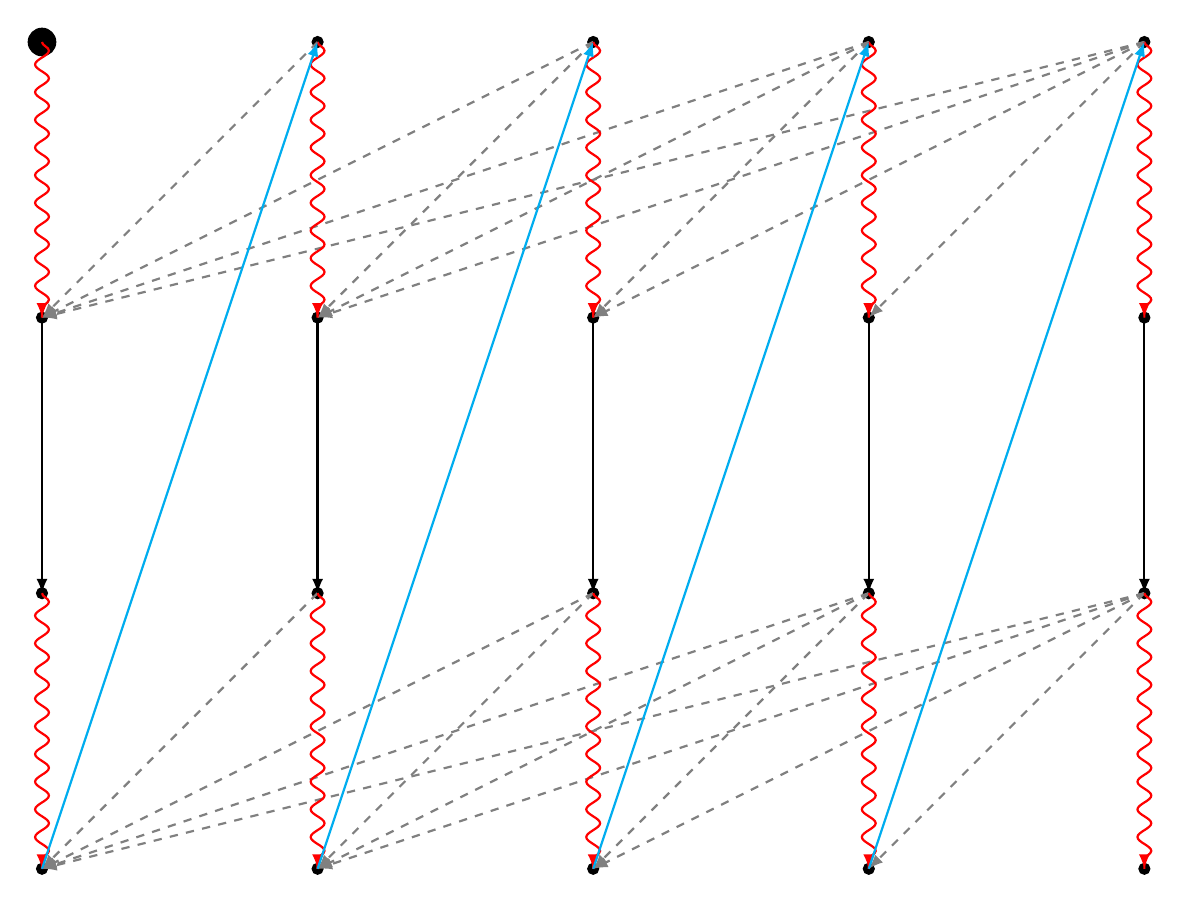
\begin{tikzpicture}[xscale=3.5,yscale=3.5]
			\draw (0,0) circle (0.05cm);
			\fill (0,0) circle (0.05cm);
			
			\foreach \x in {0,1,2,3,4}
			{
				\draw (\x,0) circle (0.02cm);
				\fill (\x,0) circle (0.02cm);
			}
			
			\foreach \x in {0,1,2,3,4 }
			{
				\draw (\x,-1) circle (0.02cm);
				\fill (\x,-1) circle (0.02cm);
			}
			
			\foreach \x in {0,1,2,3,4 }
			{
				\draw (\x,-2) circle (0.02cm);
				\fill (\x,-2) circle (0.02cm);
			}
			
			\foreach \x in {0,1,2,3,4 }
{
	\draw (\x,-3) circle (0.02cm);
	\fill (\x,-3) circle (0.02cm);
}
			
			
			
			
			\foreach \x in {0,1,2,3 }
			{
				
				
				
			}
			
			\draw[   thick, gray,dashed, -latex] (4,0) -- (3,-1);
			\draw[   thick, gray,dashed, -latex] (4,0) -- (2,-1);
			\draw[   thick, gray,dashed, -latex] (4,0) -- (1,-1);
			\draw[   thick, gray,dashed, -latex] (4,0) -- (0,-1);
			\draw[   thick, gray,dashed, -latex] (3,0) -- (2,-1);
			\draw[   thick, gray,dashed, -latex] (3,0) -- (1,-1);
			\draw[   thick, gray,dashed, -latex] (3,0) -- (0,-1);
			\draw[   thick, gray,dashed, -latex] (2,0) -- (1,-1);
			\draw[   thick, gray,dashed, -latex] (2,0) -- (0,-1);
			\draw[   thick,  gray,dashed, -latex] (1,0) -- (0,-1);
			
 
			\draw[   thick, gray,dashed, -latex] (4,0-2) -- (3,-1-2);
			\draw[   thick, gray,dashed, -latex] (4,0-2) -- (2,-1-2);
			\draw[   thick, gray,dashed, -latex] (4,0-2) -- (1,-1-2);
			\draw[   thick, gray,dashed, -latex] (4,0-2) -- (0,-1-2);
			\draw[   thick, gray,dashed, -latex] (3,0-2) -- (2,-1-2);
			\draw[   thick, gray,dashed, -latex] (3,0-2) -- (1,-1-2);
			\draw[   thick, gray,dashed, -latex] (3,0-2) -- (0,-1-2);
			\draw[   thick, gray,dashed, -latex] (2,0-2) -- (1,-1-2);
			\draw[   thick, gray,dashed, -latex] (2,0-2) -- (0,-1-2);
			\draw[   thick,  gray,dashed, -latex] (1,0-2) -- (0,-1-2);

			
			\foreach \x in {0,1,2,3,4 }
			{
				\draw [decorate,decoration=snake,thick	,red			 ] (\x,0) -- (\x,-1);
								\draw[   thick,red ,  -latex ] (\x,-1+0.05) -- (\x,-1);
																\draw[   thick ,  latex -] (\x,-2) -- (\x,-1);
																\draw [decorate,decoration=snake,thick	,red			 ] (\x,-2) -- (\x,-3);
																	\draw[   thick,red ,  -latex ] (\x,-3+0.05) -- (\x,-3);
			}
			
			\foreach \x in {0,1,2,3 }
			{
				\draw[   thick , cyan, latex -] (\x+1,0) -- (\x,-3);
			}
			
			
		\end{tikzpicture}

\end{document}